% ----------------------------------------------------------
% MODELAGEM E DEFINIÇÕES TÉCNICAS
% ----------------------------------------------------------
\section{Modelagem e definições técnicas}
Esta seção tem por objetivo demonstrar as modelagens e padronizações utilizadas no desenvolvimento da aplicação.

\subsection{Modelo Entidade Relacionamento}

\begin{figure}[H]
	\centering 
	\caption{\label{fig:mer}Modelagem Entidade Relacionamento}
	\includegraphics[width=\textwidth]{../imagens/Mer-estagiei.png} 
	\fonte{Os Autores}
\end{figure}

\subsection{Diagrama Entidade-Relacionamento}

\begin{figure}[H]
	\centering 
	\caption{\label{fig:der}Diagrama Entidade Relacionamento}
	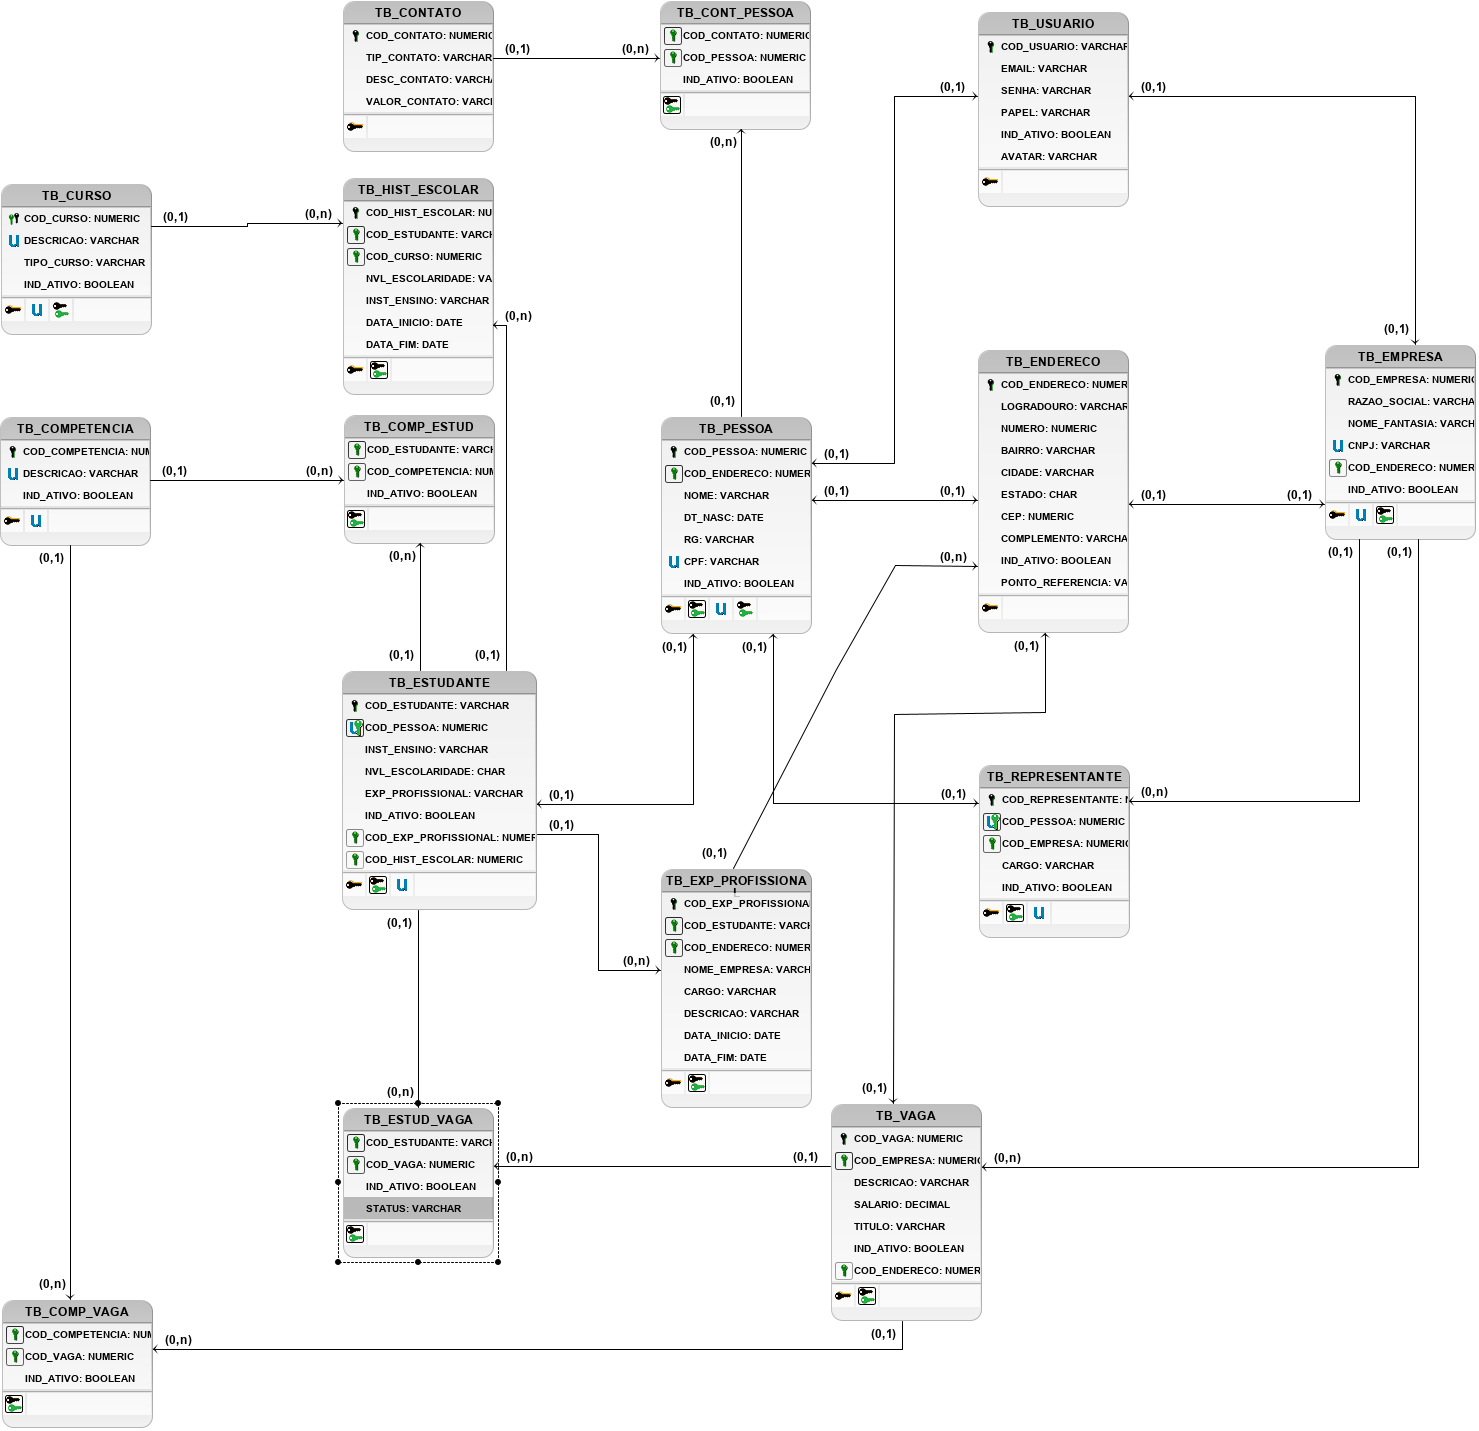
\includegraphics[width=\textwidth]{../imagens/der-estagiei.png} 
	\fonte{Os Autores}
\end{figure}

\subsection{Dicionário de Dados}
A seguir mostramos as tabelas do dicionário de dados.

\begin{quadro}[H]
	\caption{Legenda}
	\centering
	\begin{tabular}{| l | l |}
		\hline
		\thead{Sigla}	& \thead{Descrição}\\
		\hline
		PK			&   \textit{Primary Key}		\\
		\hline
		FK		    &  \textit{ Foregin Key}		\\
		\hline
		NN			&   \textit{Not Null}		\\
		\hline
		UQ			&   \textit{Unique}			\\
		\hline
		CK			&   \textit{Check}			\\
		\hline
		DEFAULT		&   \textit{Default}			\\
		\hline
	\end{tabular}
	\fonte{Os Autores}
	\label{legendas}
\end{quadro}

\begin{quadro}[H]
	\caption{Campos de Usuário}
	\centering
	\begin{tabular}{| l | l | l | p{0.3\textwidth} |}
		\hline
		\thead{Campo} & \thead{Tipo} & \thead{Restrição}	& \thead{Descrição}\\
		\hline
		Cod\_usuario    & VARCHAR      & PK      & Identificador único para usuário         \\ 
		\hline
		Senha           & VARCHAR(50)  &         & Senha de acesso                          \\ 
		\hline
		Papel           & VARCHAR(25)  & DEFAULT & Papel de acesso do usuário no sistema    \\ 
		\hline
		E-mail          & VARCHAR(50)  &         & E-mail de acesso                          \\ 
		\hline
		Avatar          & VARCHAR(100) &         & Armazenamento de imagem do perfil Google \\ 
		\hline
		Ind\_Ativo      & BOOLEAN      & DEFAULT & Indicador de estado                      \\ 
		\hline
	\end{tabular}
	\fonte{Os Autores}
	\label{campos-usuario}
\end{quadro}

\begin{quadro}[H]
	\caption{Campos de Pessoa}
	\centering
	\begin{tabular}{| l | l | l | p{0.3\textwidth} |}
		\hline
		\thead{Campo} & \thead{Tipo} & \thead{Restrição}	& \thead{Descrição}\\
		\hline
		Cod\_Pessoa   & SERIAL      & PK      & Identificador único para pessoa         \\ 
		\hline
		Cod\_Endereco & SERIAL      & FK, NN  & Chave estrangeira vinda de tb\_endereco \\ 
		\hline
		Nome          & VARCHAR(50) & NN      & Nome                                    \\ 
		\hline
		Dt\_Nasc      & DATE        & NN      & Data de nascimento                      \\ 
		\hline
		RG            & VARCHAR(11) & NN      & Registro Geral                          \\ 
		\hline
		CPF           & VARCHAR(13) & NN, UQ  & Cadastro de Pessoa Física               \\ 
		\hline
		Ind\_Ativo    & BOOLEAN     & DEFAULT & Indicador de estado                     \\ 
		\hline
	\end{tabular}
	\fonte{Os Autores}
	\label{campos-pessoa}
\end{quadro}

\begin{quadro}[H]
	\caption{Campos de Vaga}
	\centering
	\begin{tabular}{| l | l | l | p{0.3\textwidth} |}
		\hline
		\thead{Campo} & \thead{Tipo} & \thead{Restrição}	& \thead{Descrição}\\
		\hline
		Cod\_Vaga     & SERIAL      & PK      & Indicador único                 \\ 
		\hline
		Cod\_Empresa  & SERIAL      & FK NN   & Chave estrangeira de tb\_empresa  \\ 
		\hline
		Descricao     & TEXT        &         & Descrição da vaga                       \\ 
		\hline
		Salario       & FLOAT(5)    &         & Remuneração da vaga                     \\ 
		\hline
		Titulo        & VARCHAR(30) &         & Titulo da vaga                          \\ 
		\hline
		Cod\_endereco & SERIAL      & FK NN   & Chave estrangeira de tb\_endereco \\ 
		\hline
		Ind\_Ativo    & BOOLEAN     & DEFAULT & Indicador de estado da vaga             \\ 
		\hline
	\end{tabular}
	\fonte{Os Autores}
	\label{campos-vaga}
\end{quadro}

\begin{quadro}[H]
	\caption{Campos de Curso}
	\centering
	\begin{tabular}{| l | l | l | p{0.3\textwidth} |}
		\hline
		\thead{Campo} & \thead{Tipo} & \thead{Restrição}	& \thead{Descrição}\\
		\hline
		Cod\_Curso  & SERIAL      & PK      & Identificador único\\ 
		\hline
		Descricao   & VARCHAR(50) & NN, UQ  & Descrição do curso  \\ 
		\hline
		Tipo\_Curso & CHAR(1)     & NN      & Tipo do Curso) \\ 
		\hline
		Ind\_Ativo  & BOOLEAN     & DEFAULT & Indicador de estado de tb\_curso \\ 
		\hline
	\end{tabular}
	\fonte{Os Autores}
	\label{campos-curso}
\end{quadro}

\begin{quadro}[H]
	\caption{Campos de Estudante}
	\centering
	\begin{tabular}{| l | l | l | p{0.3\textwidth} |}
		\hline
		\thead{Campo} & \thead{Tipo} & \thead{Restrição}	& \thead{Descrição}\\
		\hline
		Cod\_Estudante         & VARCHAR & PK         & Identificador único  \\ \hline
		Cod\_Pessoa            & SERIAL  & FK, NN, UQ & Chave estrangeira de tb\_pessoa            \\ 
		\hline
		Cod\_Hist\_Escolar     & SERIAL  & FK, NN     & Chave estrangeira de tb\_hist\_escolar     \\ 
		\hline
		Cod\_Exp\_Profissional & SERIAL  & FK         & Chave estrangeira  de tb\_exp\_profissional \\ 
		\hline
		Ind\_Ativo             & BOOLEAN & DEFAULT    & Indicador de estado do estudante            \\ 
		\hline
	\end{tabular}
	\fonte{Os Autores}
	\label{campos-estudante}
\end{quadro}

\begin{quadro}[H]
	\caption{Campos de Empresa}
	\centering
	\begin{tabular}{| l | l | l | p{0.3\textwidth} |}
		\hline
		\thead{Campo} & \thead{Tipo} & \thead{Restrição}	& \thead{Descrição}\\
		\hline
		Cod\_Empresa   & SERIAL      & PK      & Identificador único para a empresa      \\ 
		\hline
		Razao\_Social  & VARCHAR(50) & NN      & Razão social da empresa                 \\ 
		\hline
		Nome\_Fantasia & VARCHAR(50) &         & Nome fantasia da empresa                \\ 
		\hline
		CNPJ           & VARCHAR(20) & NN, UQ  & Cadastro Nacional de Pessoas Jurídicas  \\ 
		\hline
		Cod\_Endereco  & SERIAL      & FK, NN  & Chave estrangeira vinda de tb\_endereco \\ 
		\hline
		Ind\_Ativo     & BOOLEAN     & DEFAULT & Indicador de estado da empresa          \\ 
		\hline
	\end{tabular}
	\fonte{Os Autores}
	\label{campos-empresa}
\end{quadro}

\begin{quadro}[H]
	\caption{Campos de Representante RH}
	\centering
	\begin{tabular}{| l | l | l | p{0.3\textwidth} |}
		\hline
		\thead{Campo} & \thead{Tipo} & \thead{Restrição}	& \thead{Descrição}\\
		\hline
		Cod\_Representante & SERIAL      & PK      & Identificador único                \\ 
		\hline
		Cod\_Pessoa        & SERIAL      & FK, NN  & Chave estrangeira de tb\_pessoa    \\ 
		\hline
		Cod\_Empresa       & SERIAL      & FK      & Chave estrangeira de tb\_empresa   \\ 
		\hline
		Cargo              & VARCHAR(50) & NN      & Descrição do cargo do representante \\ 
		\hline
		Ind\_Ativo         & BOOLEAN     & DEFAULT & Indicador de estado do representante   \\ 
		\hline
	\end{tabular}
	\fonte{Os Autores}
	\label{campos-rh}
\end{quadro}


\subsection{\textit{Endpoints} da API}
A seguir são apresentados os \textit{\glspl{endpoint}} mapeados até o momento, com seus respectivos métodos de requisição \gls{http}.

\begin{quadro}[H]
	\caption{\textit{\Glspl{endpoint}} de Estudante}
	\centering
	\begin{tabular}{| l | l |}
		\hline
		\thead{Método}	& \thead{\textit{Endpoint}}			\\
		\hline
		GET				& /api/estudante/\{codEstudante\}	\\
		\hline
		PUT				& /api/estudante/\{codEstudante\}	\\
		\hline
		POST			& /api/loginEstudante				\\
		\hline
		GET				& /api/estudante				\\
		\hline
		GET				& /api/estudante/\{codEstudante\}/recomendacao	\\
		\hline
	\end{tabular}
	\fonte{Os Autores}
	\label{endpoints-estudante}
\end{quadro}

\begin{quadro}[H]
	\caption{\textit{\Glspl{endpoint}} de Vaga}
	\centering
	\begin{tabular}{| l | l |}
		\hline
		\thead{Método}	& \thead{\textit{Endpoint}}	\\
		\hline
		GET				& /api/vaga	\\
		\hline
		POST			& /api/vaga	\\
		\hline
		GET				& /api/estudante/\{codEstudante\}/recomendacao	\\
		\hline
	\end{tabular}
	\fonte{Os Autores}
	\label{endpoints-vaga}
\end{quadro}


\begin{quadro}[H]
	\caption{\textit{\Glspl{endpoint}} de Empresa}
	\centering
	\begin{tabular}{| l | l |}
		\hline
		\thead{Método}	& \thead{\textit{Endpoint}}	\\
		\hline
		GET				& /api/empresa	\\
		\hline
		POST			& /api/empresa	\\
		\hline
		GET				& /api/empresa/\{codEmpresa\} \\
		\hline
	\end{tabular}
	\fonte{Os Autores}
	\label{endpoints-empresa}
\end{quadro}

\begin{quadro}[H]
	\caption{\textit{\Glspl{endpoint}} de Competência}
	\centering
	\begin{tabular}{| l | l |}
		\hline
		\thead{Método}	& \thead{\textit{Endpoint}}	\\
		\hline
		GET				& /api/competencia	\\
		\hline
	\end{tabular}
	\fonte{Os Autores}
	\label{endpoints-competencia}
\end{quadro}

\subsection{Listagem das Competências}
A seguir são apresentadas as competências parametrizadas a fim de realizar as recomendações de vagas para os estudantes de acordo com seu perfil.

\begin{itemize}
	\label{softskills}
	\item Adaptação
	\item Atitude positiva
	\item Autoconfiança
	\item Autogestão
	\item Boa escrita
	\item Capacidade de resolver problemas
	\item Capacidade de tomar decisões
	\item \textit{Coaching}
	\item Colaboração
	\item Comunicação
	\item Conhecimento político e cultural
	\item Criatividade
	\item Desenvolvimento da esquipe
	\item Desenvolvimento pessoal
	\item Empatia
	\item Estabelecimento de confiança
	\item Ética no trabalho
	\item Flexibilidade
	\item Gerenciamento de conflitos
	\item Honestidade
	\item Influência
	\item Inteligência emocional
	\item Interesse em aprender
	\item Liderança
	\item Motivação
	\item Organização
	\item Pensamento crítico
	\item Poder de negociação
	\item Proatividade
	\item Relacionamento interpessoal
	\item Resiliência
	\item Trabalho em Equipe
	\item Trabalho sob pressão
\end{itemize}